\documentclass{article}
\usepackage[utf8]{inputenc}

\usepackage{hyperref}
\usepackage{float}
%Page Margins and stuff
\usepackage{geometry}
 \geometry{
 a4paper,
 total={170mm,257mm},
 left=20mm,
 }
 
 %pictures
\usepackage{graphicx}
\graphicspath{ {./images/} }

%Multi Tab Tables
\usepackage{multirow}

%Move the title position
\usepackage{titling}

\setlength{\droptitle}{-7.7em} %Up, near the top but not too high

\title{Computing Systems Assignment 4 - Finite State Machines}
\author{Daniel Hannon (19484286)}
\date{February 2020}

\begin{document}

\maketitle

\begin{figure}[h!]
	\centering
	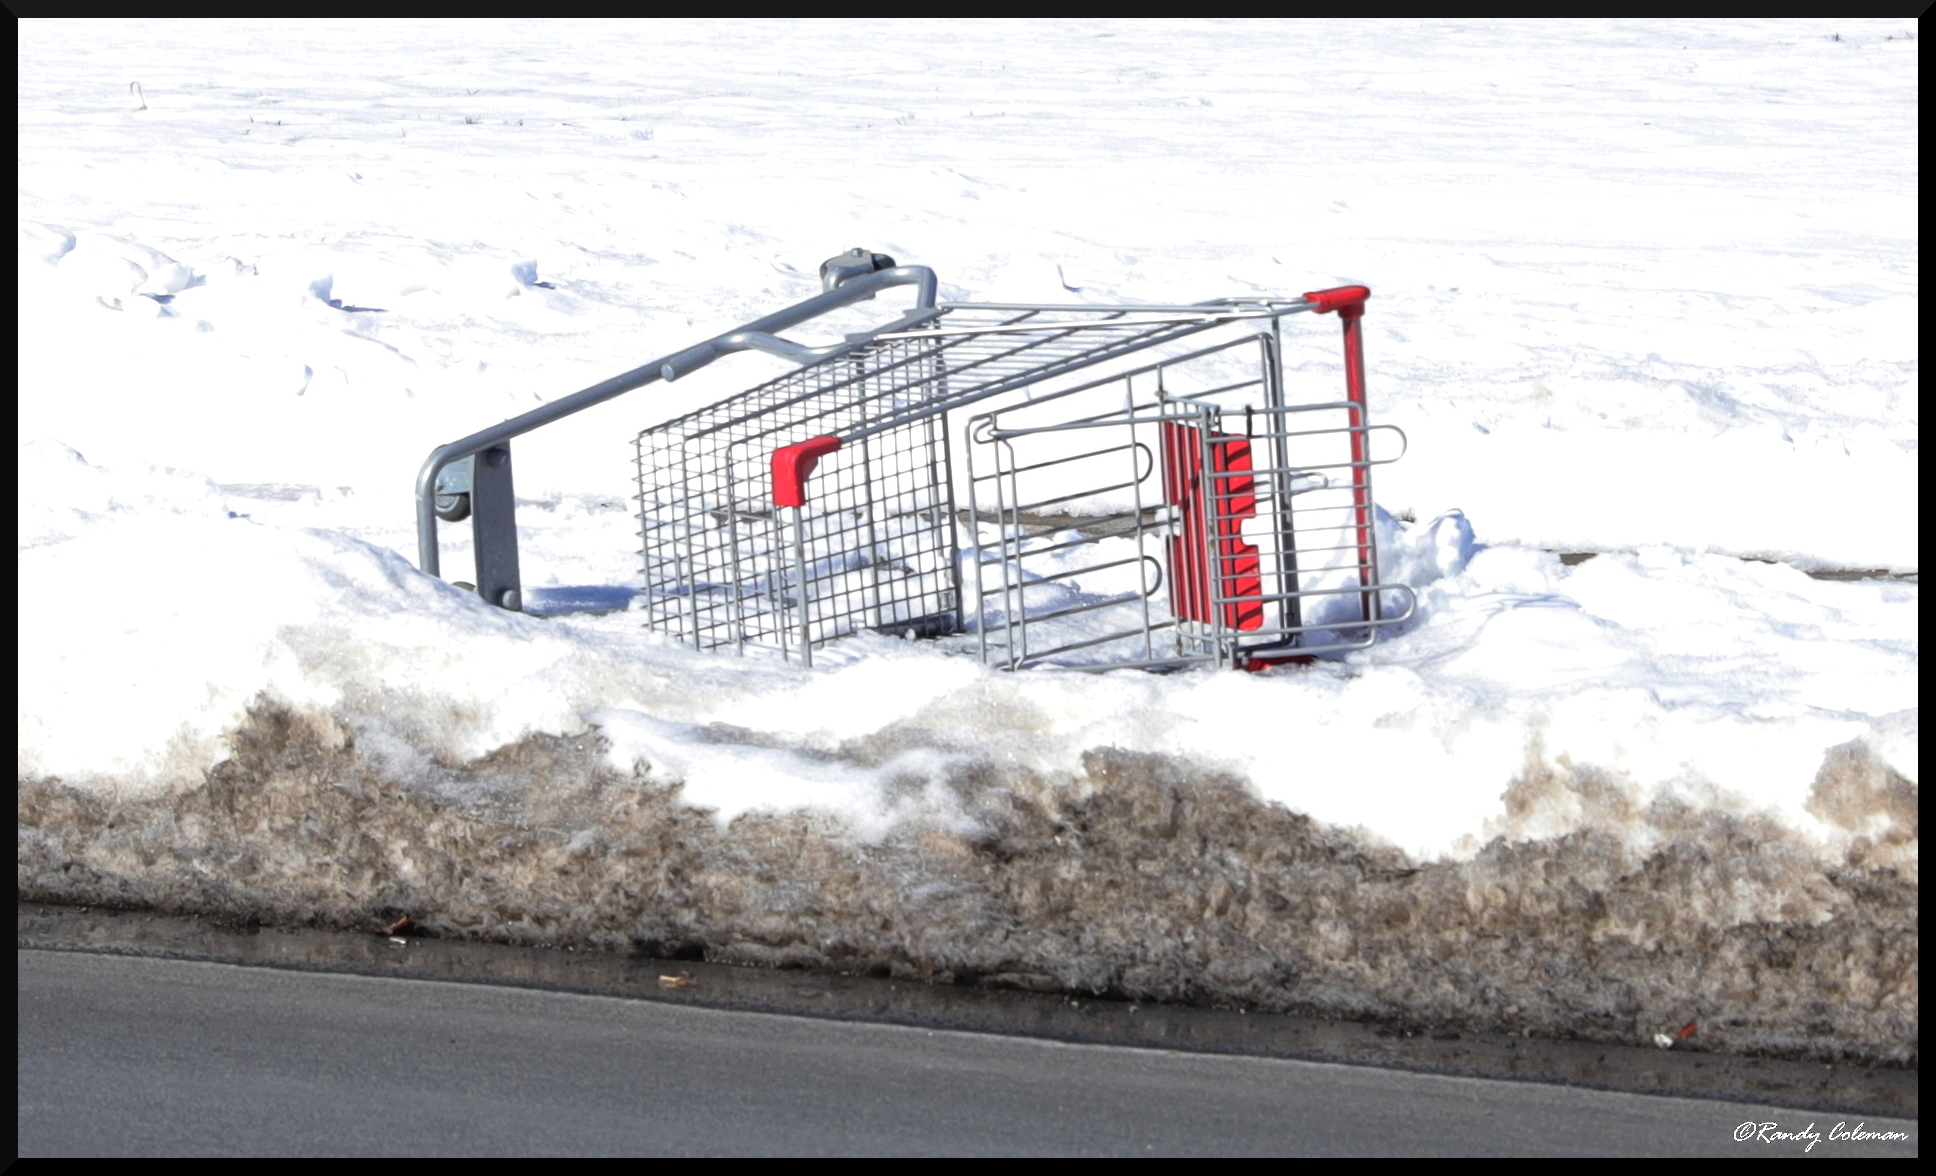
\includegraphics[scale=0.24]{images/cover-trolley.jpg}
	\caption{The Lock on this trolley is An Example of A Finite State Machine. Source: Twitter @Wagerlkunst}
	\label{fig:trolley}
\end{figure}

\section{Introduction}
Finite State Automata or Finite State Machines are one of the key components of a computer. In order for a computer to exist be it conceptual or physical, it must have some ability to deal with changes in inputs and alter outputs as such.
\\ Within the contents of this report I hope to achieve the following:
\begin{enumerate}
	\item Give a general overview and history of Finite State Machines(FSM)
	\item Distinguish between the Mealy and Moore types of Finite State Machines.
	\item Give a fully conceptualized example of a Finite State Machine.
\end {enumerate}

\section{What is an FSM?}
\subsection{Overview}
A Finite State Machine (or FSM for short) is a tool which is often used to model the behaviour of a sequential system such as an Elevator. They consist of numerous states. The next state in which the machine will go to is determined by:
\begin{itemize}
	\item The Inputs going into the machine.
	\item The Current state of the machine
\end {itemize}
\newpage
\subsection{History of the Finite State Machine}
\begin{figure} [h!]
	\centering
	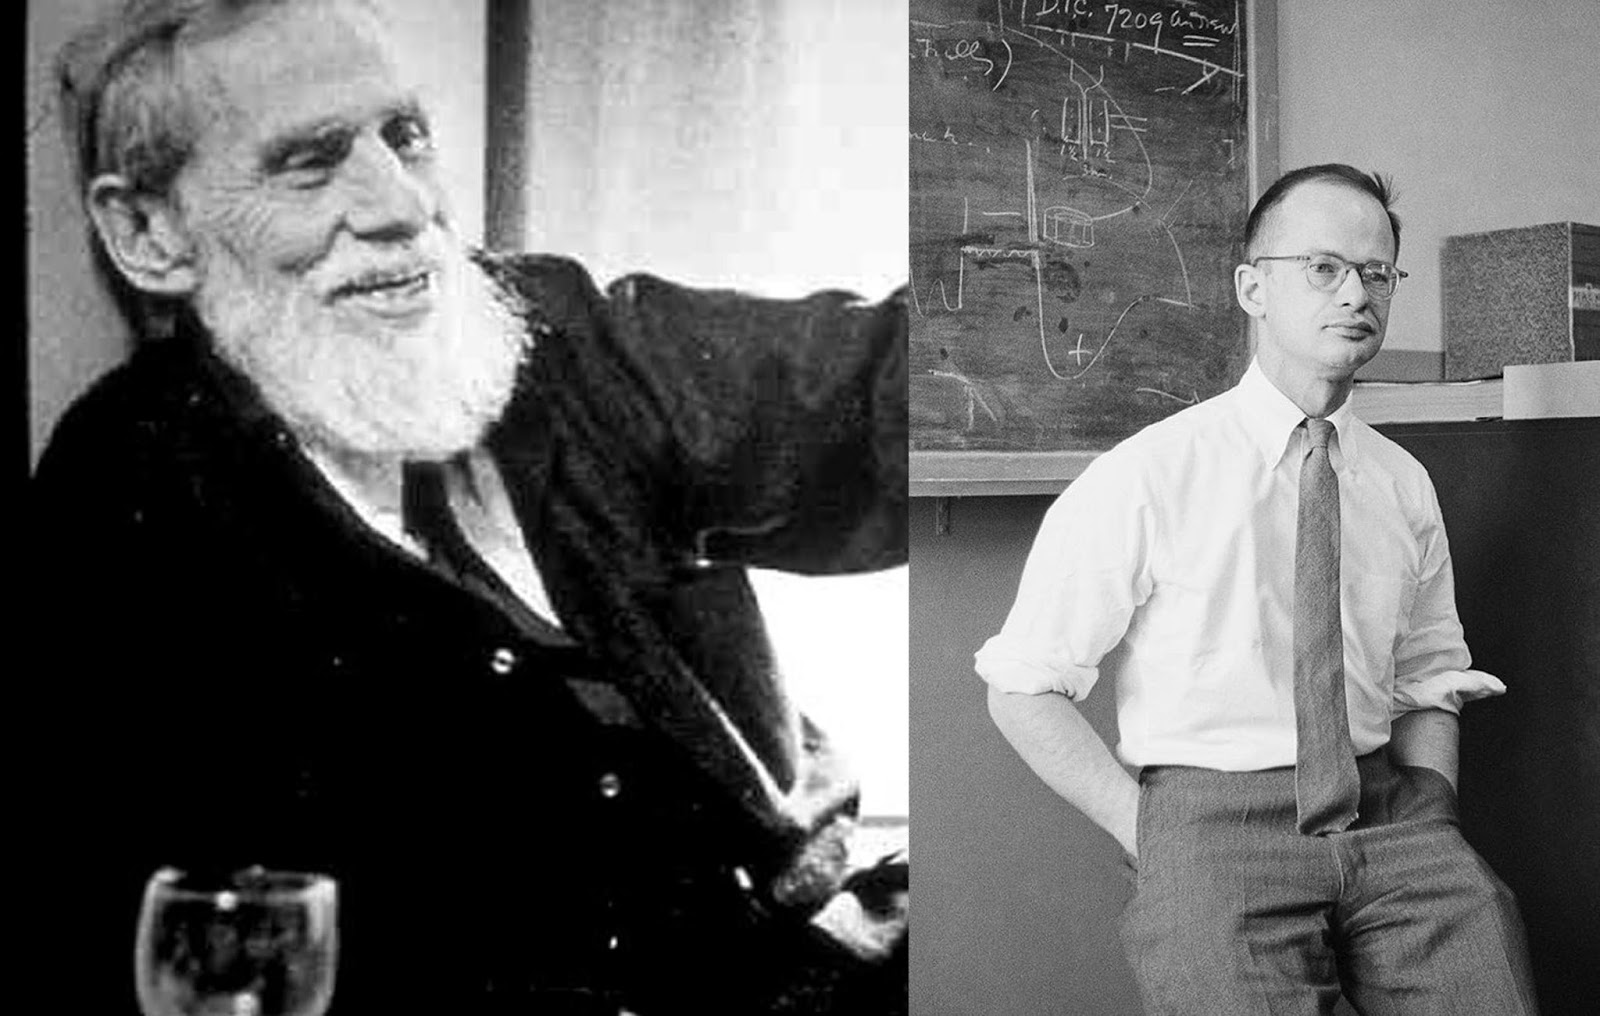
\includegraphics[scale=0.1]{mccullochpitts.jpg}
	\caption{McCulloch (left) and Pitts (right)}
	\label{fig:fsm}
\end{figure}
Finite State Machines are not wholly restricted to computer science. In fact the groundwork for the theory of finite state automata was written by academics from numerous fields, Including but not limited to: Biology, Psychology, Mathematics, Engineering, and of course Computer Science. 
\par\null\par
All of these academics were motivated by one common goal: to accurately model the Human Thought Process. 
One of the first defining papers for Finite State Machines as we know them today were set out in a 1943 paper titled "A Logical Calculus Immanent in Nervous Activity" Which was written by two Neurophysiologists called Warren McCulloch and Walter Pitts. This paper made extremely large contributons to the study of Neural Networks, Automata, and Cybernetics. It was not until the 1950's when G.H. Mealey and E.F. Moore, in separate papers applied the work to far more powerful machines that it truly made an impact in the field. There are a few notable differences between what Mealy and Moore defined as a Finite State Machine, and we will explore these in Section 2 of this report.
\subsection{What are Finite State Machines Used For?}
Finite State Machines are used for many things in everyday life, everything from a trolley lock to an elevator is are Finite State Machines. some very good examples of Finite State Machines are as follows:
\begin{itemize}
	\item Vending Machines - They have the number pad and cash inserted as an input and food as an output 
	\item Automated Teller Machines - These work similarly to a vending machine but they allow you to perform menial/mundane tasks with your bank account such as, checking your balance, changing your pin, depositing money, and withdrawing money. they are often employed as a means of both accelerating banking operations and of reducing the required workforce to perform basic teller duties.
	\item Security Systems - such as fire alarms, burgular alarms, automatic locks, and Emergency Lighting systems.
	\item Assistive Technologies - Power assisted doors, chair lifts, and alarms. 
\end {itemize}
\subsection{Basic Example of a Finite State Machine}
In order to explain a Finite State Machine we will return to \figurename{\ref{fig:trolley}} where there is an image depicting an out of comission shopping trolley. The lock on the shopping trolley is a great example of a very basic Finite State Machine. O1 refers to a state change while O2 refers to a looping action
\begin{figure}[h!]
	\begin{minipage}[t]{0.48\linewidth}
		\vspace{0pt}
		\centering
		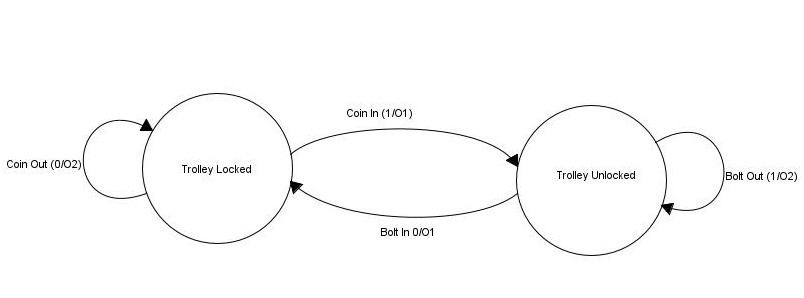
\includegraphics[scale = 1]{trolley-fsm.jpg}
	\end{minipage}
	\begin{minipage}[t]{0.48\linewidth}
		\vspace{0pt}
			\centering
			\resizebox{0.75\columnwidth}{!}{%
			\begin{tabular}{|l|l|l|l|l|}
				\hline
				\multicolumn{1}{|c|}{\multirow{2}{*}{State}} & \multicolumn{2}{c|}{Input = 0} & \multicolumn{2}{c|}{Input = 1} \\ \cline{2-5} 
				\multicolumn{1}{|c|}{}                       & Next State       & Output      & Next State       & Output      \\ \hline
				S1                                           & S1               & O2          & S2               & O1          \\ \hline
				S2                                           & S1               & O1          & S2               	& O2          \\ \hline
			\end{tabular}
			}
	\end{minipage}
	\caption{Trolley Finite State Machine and State Table}
	\label{fig:trolleyfsm}
\end{figure}
\\ Based on the information above, hopefully I have made it clear that a Finite State Machine changes states depending on change in input. 
\section {Mealy versus Moore}
As Mentioned before, there are two main types of Finite State Machine which we look at when it comes to computational theory. Mealy Machines, and Moore Machines.
\subsection{Mealy Machine}
\subsubsection{History of a Mealy Machine}
In 1955 George H. Mealy, published a paper titled "A Method for Synthesizing Sequential Circuits" in which he outlined the Mealy Machine as we know it today.
\subsubsection{Overview of a Mealy Machine}
A Mealy Machine is defined as a machine whose output values are determined by both its current state and its input values. The Machine described in \figurename{\ref{fig:trolley}} and \figurename{\ref{fig:trolleyfsm}} is of course a Mealy machine as the state of the trolley lock mechanism was entirely dependent on the inputs that were present as well as the current state of the trolley. Below is a diagram for a sequence detector for 01 or 10 With an accompanying table. 
\begin {figure}[H]
	\begin{minipage}[t]{.48\linewidth}
		\vspace{0pt}
		\centering
		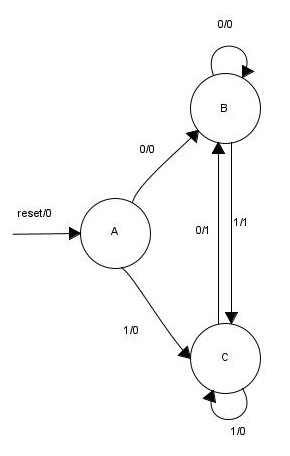
\includegraphics[scale = 1.5]{berkley-mealy.jpg}
	\end{minipage}
	\begin{minipage}[t]{.48\linewidth}
		\vspace{0pt}
		\begin{tabular}{c c c | c c}
			&	&	Current & Next	&	\\
			Reset & Input & State & State & Output\\
			\hline
			1 & - & - & A & 0 \\
			0 & 0 & A & B & 0 \\
			0 & 1 & A & C & 0 \\
			0 & 0 & B & B & 0 \\
			0 & 1 & B & C & 1 \\
			0 & 0 & C & B & 1 \\
			0 & 1 & C & C & 0 \\
		\end{tabular}
	\end{minipage}
	\label{fig:berkley-fsm-mealy}
	\caption{Mealy Machine Diagram and State Table}
\end {figure}
\subsection{Moore Machine}
\subsubsection{History of the Moore Machine}
In 1956, Edward F. Moore presented his take on the Finite State Machine in a paper titled "Gedanken-experiments on Sequential Machines"
\subsubsection{Overview of the Moore Machine}
Contrary to the Mealy Machine, a moore machines outputs are determined entirely by it's current state and I will provide a diagram of a sequence detector for 01 or 10 along with an accompanying table. 
\begin{figure}[H]
	\begin{minipage}[t]{0.48\linewidth}
		\vspace{0pt}
		\centering
		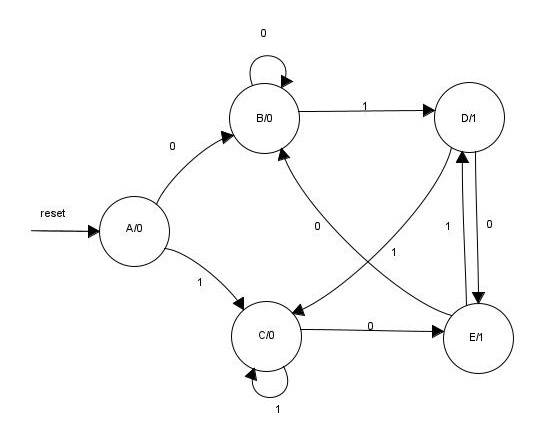
\includegraphics[scale = 1.5]{berkley-moore.jpg}
	\end{minipage}
	\begin{minipage}[t]{0.48\linewidth}
		\vspace{0pt}
		\begin{tabular}{c c c | c c} 
			& & Current & Next & \\
			Reset & Input & State & State & Output \\
			\hline
			1 & - & - & A & \\
			0 & 0 & A & B & 0 \\
			0 & 1 & A & C & 0 \\
			0 & 0 & B & B & 0 \\
			0 & 1 & B & D & 0 \\
			0 & 0 & C & E & 0 \\
			0 & 1 & C & C & 0 \\
			0 & 0 & D & E & 1 \\
			0 & 1 & D & C & 1 \\
			0 & 0 & E & B & 1 \\
			0 & 1 & E & D & 1 \\
		\end {tabular}
	\end{minipage}
	\label{fsm:berkley-moore}
	\caption{Moore Machine and State Table}
\end{figure}
\newpage
%%BIG MAN TINGZ BELOW
\section {Worked Example of a somewhat complex Finite State Machine}
\subsection{Overview of the Finite State Machine of choice}
For my Finite State Machine I have selected a 4-digit combination lock. Due to the fact that the lock would in reality would have 100,000,000 combinations as the passcode mechanism would consist of 4 sets of mod 10 counters as one would be required to keep track of the position of the pin in the barrel and another would be required to keep track of the digit displayed to the end user.\\
A way to reduce it to 10,002 states would be by making the pin have a fixed location relative to the display. Due to the fact that 100,000,002 and 10,002 are both very difficult to neatly represent, I have completely Omitted the mechanism determining the position of the pin, reducing it to a single bit for each barrel.
\par\null\par
Due to this omission it has become a significantly easier to represent, in fact it only requires 4 bits to determine state, three of which for current state, and a forth to determine whether or not the pin is in place or the bolt of the lock is open or not. Here is the now condensed state of the combination lock in table and graphic format
\par\null\par
\begin{minipage}[t]{0.48\linewidth}
	\vspace{0pt}
	\begin{tabular}{c|c||c}
		Current State & U & Next State\\
		\hline
		000 & 0 & 000 \\
		000 & 1 & 001 \\
		001 & 0 & 000 \\
		001 & 1 & 010 \\
		010 & 0 & 000 \\
		010 & 1 & 011 \\
		011 & 0 & 000 \\
		011 & 1 & 100 \\
		100 & 0 & 000 \\
		100 & 1 & 101 \\
		101 & 0 & 000 \\
		101 & 1 & 101 \\  
	\end{tabular}
\end{minipage}
\begin{minipage}[t]{0.48\linewidth}
	\vspace{0pt}
	\centering
	States represented in binary format \\
	Locked = 000\\
	Row 1 = 001\\
	Row 2 = 010\\
	Row 3 = 011 \\
	Row 4 = 100\\
	Unlocked = 101
	\par\null\par
	What "U" Represents \\
	Locked = Button\\
	Unlocked = Bolt\\
	Rows 1-4 = if pin from mod 10 is in place.
\end{minipage}
\begin{figure}[h!]
	\centering
	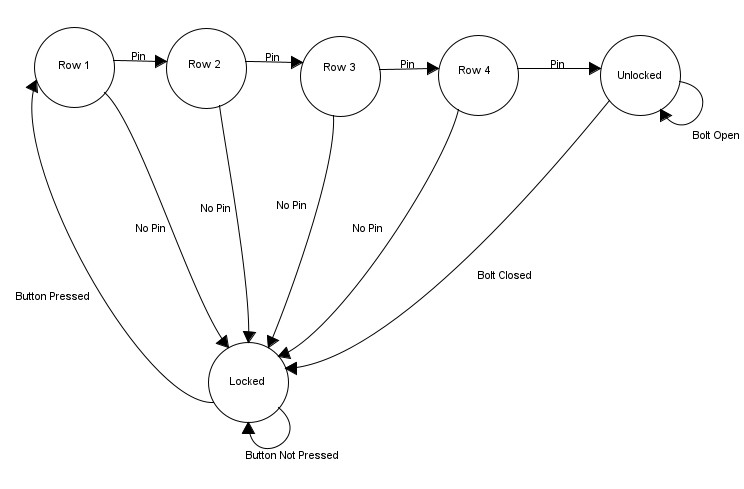
\includegraphics[scale = 0.6]{comb-lock-fsm.jpg}
	\caption{Simplified State Diagram for a Combination Lock.}
	\label{fig:comb-lock}
\end{figure}
\newpage
\subsection{Next state Logic of the FSM}
Here are the karnaugh maps which I used to create the combinational logic featured at the very bottom. the groupings have been marked in red.
\begin{figure}[h!]
	\centering
	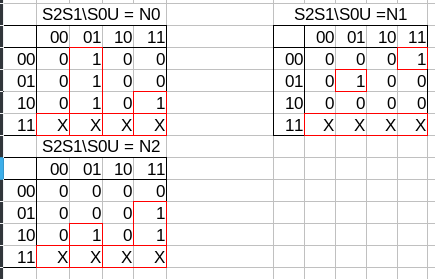
\includegraphics{karnaughmapswithgroupings.png}
	\caption{Karnaugh Maps}
	\label{}
\end{figure}
\subsection{Combinational Logic of FSM}
\begin{figure}[h!]
	\centering
	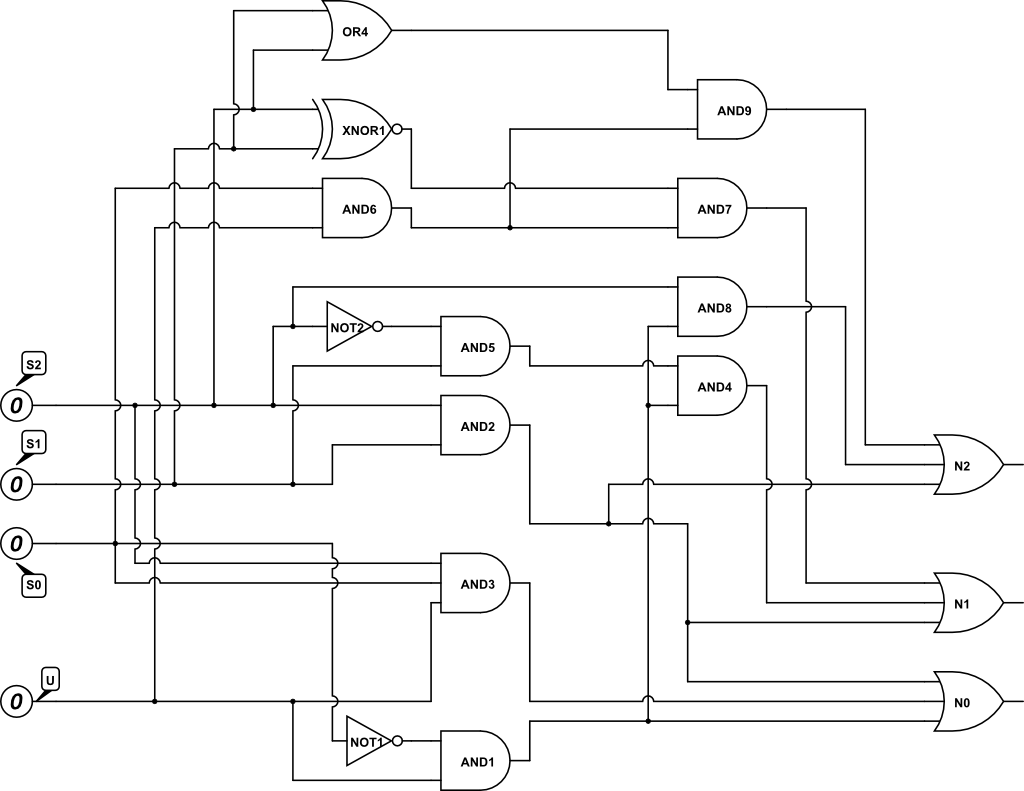
\includegraphics[scale = 0.75]{logic-circuit-fsm.png}
	\caption {Combinational Logic of Combination Lock}
	\label{fig:comblocklogic}
\end{figure}
\newpage
\section{References}
FSM Design Tool\\
fizzim.com\\

History of Finite State Machines/Mealey Moore Machines\\
https://cs.stanford.edu/people/eroberts/courses/soco/projects/2004-05/automata-theory/basics.html\\
https://www.geeksforgeeks.org/difference-between-mealy-machine-and-moore-machine/\\
Examples of Mealy and Moore Machines \\
http://www-inst.eecs.berkeley.edu/~cs150/fa05/Lectures/07-SeqLogicIIIx2.pdf
\\
McCulloch and Pitts picture \\
https://infonintelli.blogspot.com/2017/11/psychon-and-mcculloch-pitts-neurons.html\\
\end{document}